Относительно AVL"=дерева балансировкой вершины называется операция,
которая в случае разницы высот левого и правого поддеревьев $= 2$,
изменяет связи предок-потомок в поддереве данной вершины так,
что разница становится $ \leqslant 1$, иначе ничего не меняет.
Указанный результат получается вращениями поддерева данной вершины.

Используется 4 типа вращений:

\subsection*{Малое левое вращение}

%картинка 1
\begin{figure}[ht]
    \includegraphics[width = \textwidth]{1.pdf}
    
    \caption{Схематическое изображение малого левого вращения}    
\end{figure}

Данное вращение используется тогда,
когда (высота $b$"=поддерева; $L$ "--- высота )
$= 2$ и высота $С \leqslant$ высота $R$.

\subsection*{Большое левое вращение}

%картинка 2
\begin{figure}[ht]
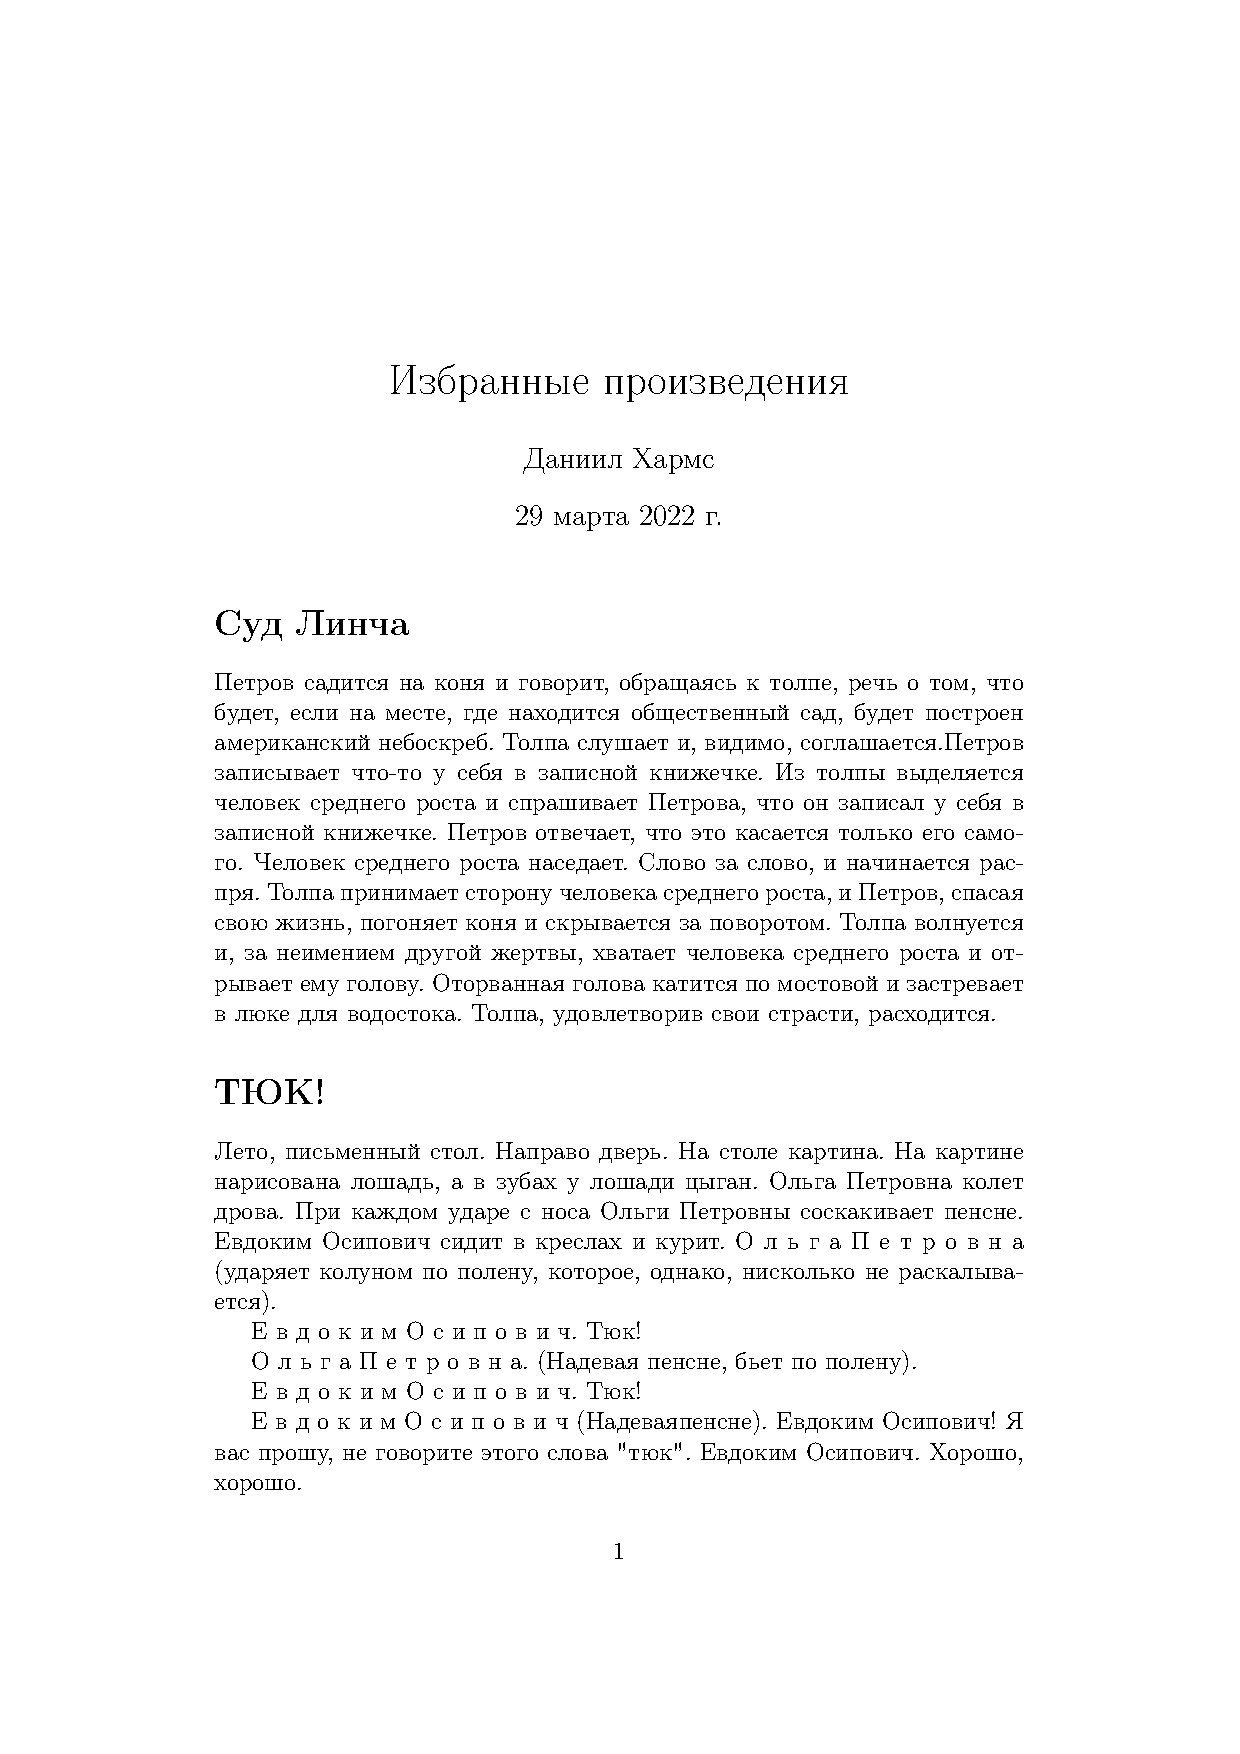
\includegraphics[width = \textwidth]{2.pdf}

\caption{Схематическое изображение большого левого вращения}
\end{figure}

Данное вращение используется тогда,
когда (высота $b$"=поддерева; $L$ "--- высота)
$= 2$ и высота $c$"=поддерева $>$ высота $R$.

\subsection*{Малое правое вращение}

%картинка 3
\begin{figure}[ht]
    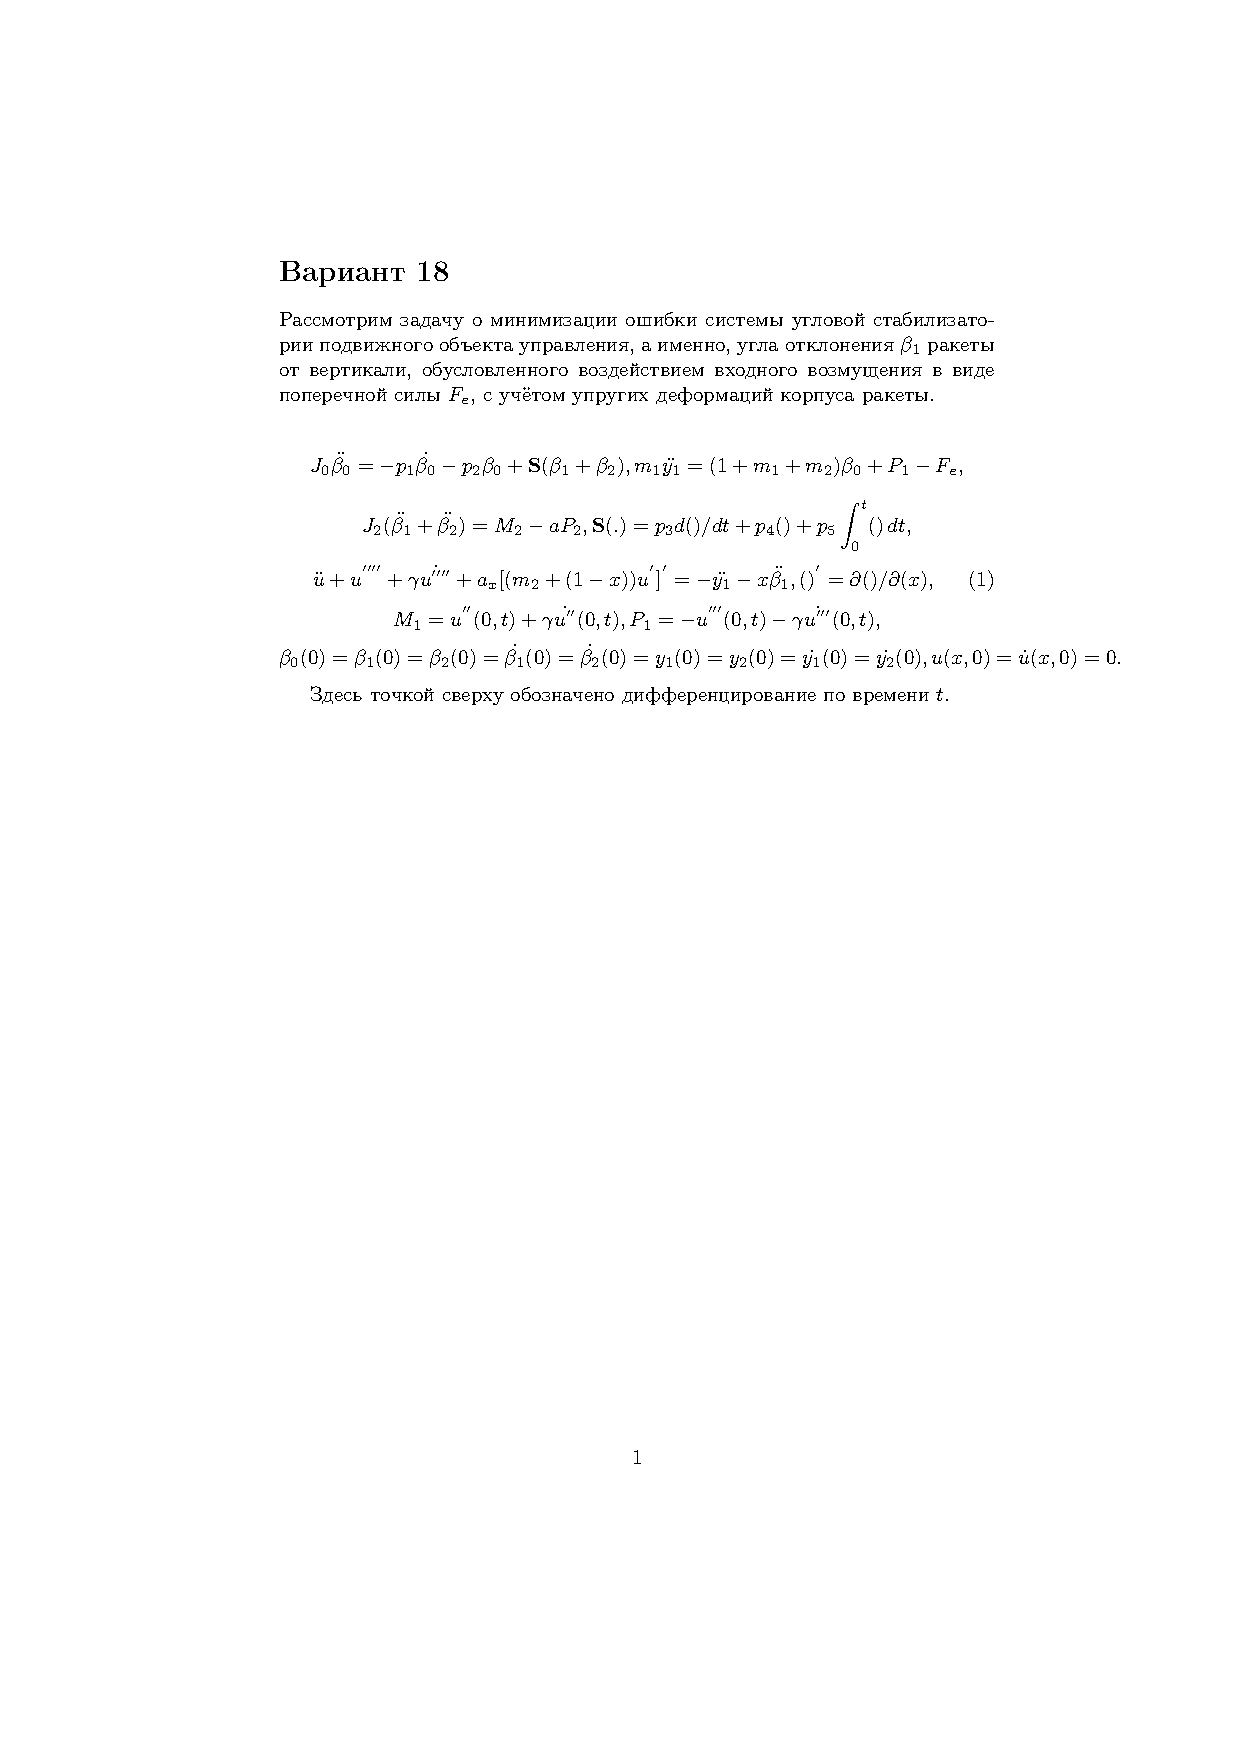
\includegraphics[width = \textwidth]{3.pdf}
    
    \caption{Схематическое изображение малого правого вращения}
\end{figure}

Данное вращение используется тогда,
когда (высота $b$"=поддерева "--- высота $R$)
$= 2$ и высота $С \leqslant $ высоты $L$.

\subsection*{Большое правое вращение}

%картинка 4
\begin{figure}[ht]
    \includegraphics[width = \textwidth]{4.pdf}
    
    \caption{Схематическое изображение большого правого вращения}

\end{figure}

Данное вращение используется тогда, когда (высота $b$"=поддерева; $R$ "--- высота)
$= 2$ ивысота $c$"=поддерева $ > $ высота $L$.
В каждом случае достаточно просто доказать то, 
что операция приводит к нужному результату и
что полная высота уменьшается не более чем на $1$ и не может увеличиться.
Из-за условия сбалансированности высота дерева $O(\lg(N))$,
где $N$ "--- количество вершин, поэтому добавление элемента требует $Q(\lg(N))$ операций.